\documentclass[a4paper,12pt]{article}
\usepackage[numbers]{natbib}
\setcitestyle{numbers}
\usepackage{mathtools}
\usepackage[toc,page]{appendix}
\usepackage{makecell}
\usepackage{graphicx}
\usepackage{caption}
\usepackage{siunitx}
\captionsetup[figure]{font=small}
\usepackage{wrapfig}
\begin{document}

\title{Parametrized cost of attack as a measure of Decred network security}
\author{Brian Stafford}
\maketitle

\section{Introduction}

Due its hybrid concensus protocol, the Decred blockchain presents unique challenges to the measurement of attack resiliency. In addition to new proof-of-stake related vulnerabilities, the well known 50\% hashpower threshold is not constant for Decred. The hashpower threshold also depends on the fraction of stake pool tickets the attacker controls. For an attacker who controls very few tickets, the hashpower threshold is very nearly 100\%, but becomes lower with increasing stake (figure \ref{sigmafig}). 

% \cite{POA}

Proposed here is a measure of network security tentatively named the \emph{parametrized cost of attack} (PCA), defined roughly as the fiat expenditure required to perform a majority attack. 

Attempts are made below to minimize the PCA, but there are certainly other ways that are not considered here. For example, access to sub-retail equipment, as in the case of a malicious chipmaker, is not considered. Denial-of-service attack components are also not considered, although they certainly deserve attention. 

\section{Ticket fraction and work fraction}
The PCA can be broken into two components; the work component, $W$ and the stake component $S$. The cost of attack, $A$, is the sum of the components.
%
\begin{equation}
A = W + S
\end{equation}
%
These two components are not independent. They are related through $ \sigma(y) $, which is the fraction of total network hashrate an attacker would need to control in order to perform an attack, given they control fraction $ y $ of the stakepool tickets. If N ticket holders are chosen per block, the probability $ P(y) $ that the attacker holds a majority of selected tickets is given by 
%
\begin{equation}
P(y) = \sum_{k=0}^{k < N/2}  {{N}\choose{k}}   y^{N-k} \Big( (1-y) \cdot p \Big)^k
\end{equation}
%
where $ {{N}\choose{k}}  $ is a binomial coefficient. $ N $ is set to 5 for Decred, but is left as a paremeter here. The participation ratio, $ p $, is the fraction of stakeholders online and ready to vote, and has historically been very nearly 1. While participation will be taken to be 1 for the remainder of this work, it is important to note that $ p $ could potentially be a target for a denial-of-service attack component. 

The attacker would hold the majority of tickets derived from every $ 1 / P(y) $ valid nonces they are able to generate. Conversely, the honest nodes would be able to achieve consensus on every $ 1 / (1 - P(y)) $ blocks proposed to the honest network. The attacker would need a factor of 
%
\begin{equation}
x(y) = \frac{ 1 / P(y) }{ 1 / ( 1 - P(y) ) } = \frac{ 1 }{ P(y) } - 1
\end{equation}
%
\begin{wrapfigure}{l}{0.50\textwidth}
  \vspace{-10pt}
  \begin{center}
    	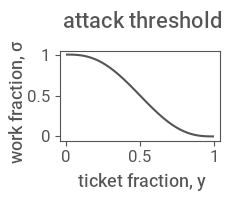
\includegraphics[width=0.34\textwidth]{sigma}
	\vspace{-10pt}
	\begin{minipage}[t]{0.35\textwidth}
	\caption{The threshold of hashpower needed to initiate an attack. \label{sigmafig}}	
	\end{minipage}
	\vspace{0pt}
  \end{center}
\end{wrapfigure}
%
times the honest hashpower in order to outpace the honest chain. There is an implicit assumption in $ x(y) $ that the attacker's hashpower is not already part of the existing honest hashpower before the attack. If this assumption is dropped, the hashpower threshold can be minimized further. Stated otherwise, assume that the attacker's hashpower is already mining honestly on the main chain before being apruptly redirected to the attacker's chain. Then
%
\begin{equation}
\label{sigmaeq}
\sigma(y) = \frac{ x(y) }{ x(y) + 1 } = 1 - P(y)
\end{equation}
%
is the fraction of total network hashrate an attacker would need to redirect to initiate an attack. 

If the network hashrate, $ H_{net} $, is known, one could use $ x(y) $ to calculate how much hashing power an attacker would need to control, and subsequently estimate how much it would cost to purchase and/or rent. 


\section{Work term}

The work term, $W$, is the cost associated with POW mining. The form of the work term is complicated by the availability of rental equipment, and so depends on market rental prices and rental availability. The general form is
%
\begin{equation}
W =  \underbracket{R}_{\text{rental}} + \underbracket{D + P}_{\text{retail}}
\end{equation}
%
where $R$ is the total costs associated with rental equipment, $D$ is the total cost of purchasing retail devices and associated equipment, and $P$ is the total cost of power over the duration of attack. $ P $ is typically small. Rental costs can be calculated given a rental price, $r_e$, (units price/hash) and a "rentability", $a$,  which represents the total rental hashing power available in units of hashrate. For an attack of duration $t_a$, the rental costs are 
%
\begin{equation}
R = a r_e t_a.
\end{equation}
%
with the condition that $ a \le H_a $. 

If there is not enough rentability to meet the attacker's hashpower threshold, retail equipment supplies the remainder. To calculate retail costs, key equipment parameters can be estimated from the device performance and retail market price of hardware. Devices will have a hashrate $h_d$, a power draw $\omega_d$, and a retail cost $p_d$. The device can be modeled after a single state-of-the-art device, or parameters can be estimated based on a survey of market conditions and history. Modeling on the state-of-the-art device typically minimizes the cost, and is the method used here. If desired, an adjustment could be added to the retail price to account for support equipment, i.e. power supplies, networking hardware, etc. 

Device parameters can also be expressed in terms of the power efficiency $\eta = h_d / \omega_d$, and relative cost $\rho = p_d / h_d$. The full retail costs are given by summing the equipment term
%
\begin{equation}
D = ( H_a - a )  \cdot \rho
\end{equation}
%
with the power term
%
\begin{equation}
P = \frac{ ( H_a - a ) }{ \eta } \cdot c \cdot t_a
\end{equation}
%
where $H_a$ is the required attacker hashrate and $c$ is the electricity rate (cost/energy). 

The attacker's required hashrate, $ H_a $, is related to the full network hashrate,  $H_{net}$, through equation \ref{sigmaeq} as 
%
\begin{equation}
H_a = \sigma(y)H_{net}.
\end{equation}
 

For further parametrization, it's useful to note the relationship between network hashrate, fiat exchange rate $ X $, miner profitability $ \alpha_w $, and various network and device parameters (see appendix A).
%
\begin{equation}
H_{net} = \frac{ \beta X }{ \alpha_w \rho + 0.024 c / \eta  }
\end{equation}
%
where $\beta$ is the total POW rewards (DCR) payed out daily. The benefit of parametrizing in terms of miner profitability is that the value is self-regulating and tends towards zero, allowing predictions of long-term behavior in a stable market. $\beta$ is dependent on various network parameters as
%
\begin{equation}
\beta = \frac{ 86400 R_{pow} }{ t_b } 
\end{equation}
%
with $R_{pow}$ the POW block reward, and $t_b$ is the network's target block time. The full block reward, $R_{tot}$, for Decred is dependent on block height, $h$.
%
\begin{equation}
R_{tot}(h) = 31.19582664(100/101)^{floor(h/6144)}
\end{equation}
%
At the time of writing, the POW miner is rewarded with 60\% of the total block reward, though it will be left as a parameter, $ s_w $, here; $R_{pow} = s_w R_{tot}$. 

The fully parametrized work term is then 
%
\begin{equation}
W = ar_et_a +\Big( H_a - a \Big) \Big(\rho + \frac{ c t_a }{ \eta } \Big)
\end{equation}
%
with
%
%
\begin{equation}
\label{hafig}
H_a = \sigma(y) \frac{ 86400 s_w R_{tot} X }{ t_b (\alpha_w \rho + 0.024 c / \eta) }
\end{equation}
%
Equation \ref{hafig} assumes units of seconds for block time and fiat/kWh for electricity rate.


\section{Stake term}
%
\begin{figure}[!b]
\hrule
	\vspace{5pt}
	\begin{center}
	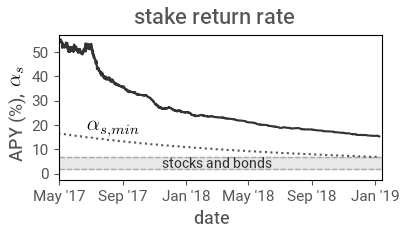
\includegraphics[width=0.62\textwidth]{stakereturn}
\begin{minipage}[t]{0.85\textwidth}
	\caption{As Decred staking gains acceptance as an investment product, the returns are approaching those of other common investment products. \label{stakereturnfig}}
	\end{minipage}
  	\end{center}
\end{figure}
%
The ticket fraction, $y$, is the ratio of attacker controlled tickets to all tickets in the stake pool. For an average stake difficulty (ticket price), $ p_t $, and a ticket pool size of $ Z $ tickets, the stake term is expressed as 
%
\begin{equation}
S = yZXp_t
\end{equation}
%
%
\begin{figure}[h]
	\begin{center}
	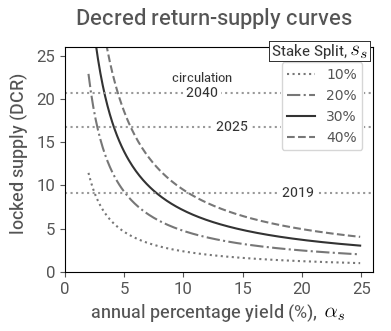
\includegraphics[width=0.55\textwidth]{returnsupply}
\begin{minipage}[t]{0.85\textwidth}
	\caption{There is a lower limit to the steady-state APY where the total stake is equal to the total supply. The position of the limit can be modified by increasing or decreasing the fraction of the block reward given to ticket holders. \label{returnsupplyfig}}
	\end{minipage}
  	\end{center}
	\hrule
\end{figure}
%
Historically, the stake difficulty has shown relative stability, even through chaotic market changes, so variations in the ticket term have mostly followed the fiat exchange rate. 

Similar to the method used on the work term, the stake term can be further parametrized by noting the relationship between ticket price, block reward, and stake annual percentage yield (APY), $ \alpha_s $, expressed as
%
\begin{equation}
\alpha_s = \bigg( \frac{ p_t + (R_{pos} / N) }{ p_t } \bigg)^{365/28} - 1
\end{equation}
%
with $ R_{pos} = s_s R_{tot} $ ($ s_s $ is currently set at 0.3). Here again, a type of profitability is chosen for parametrization due to its tendency towards some natural value. APY in particular is chosen for convenience of comparison with other investment products. Contrary to equilibrium value of $ \alpha_w $, the asymptotic value of $ \alpha_s $ is not zero. As shown in figure \ref{stakereturnfig}, as Decred staking gains acceptance as an institutional investment product, the return rate approaches the rates of other common investments. The typical APY of institutional investment products ranges from around 2\% for bonds to about 7\% for stocks. Because of the limited supply of Decred, there is also a hard lower limit on the steady-state APY possible when $ p_t = C(t) / Z $,
%
\begin{equation}
\alpha_{s, min} = \Big[ \frac{ Z R_{pos} }{ C(t) N } + 1 \Big]^{365/28} - 1
\end{equation}
%
where $ C(t) $ is the total Decred in circulation. This provides a lower limit to the valid range of $ \alpha_s $, illustrated as a dotted line in figure \ref{stakereturnfig}. 


The stake term is expressed fully as

\begin{equation}
S = \frac{ yZXs_sR_{tot} }{ N [ ( \alpha_s + 1)^{28/365} - 1 ] }
\end{equation} 

\section{Application}

To make use of the PCA, typically a starting position in parameter space is chosen, and parameters are varied one or two at a time around that position, treating all others as either constant, or changing in some known way with the chosen variable(s). For the sake of the following examples, the starting position is chosen to be the conditions at the time of writing ($ \chi = 17.5, \alpha_s = 0.153, h=309,000 $), though the general trends are valid over a wide range of conditions.

To demonstrate the application of the relations developed above, an attempt is made here to investigate a couple of common questions. 

\subsection{Which mining algorithm provides the highest network security? }

At all but the highest rentabilities, the retail equipment term dominates the PCA. Using the relations developed in the appendix, it can be shown that at a given exchange rate, the retail capital, $ C_{retail} = W / \sigma(y) = N_d \cdot p_d $, of devices on the network depends only on the price and power consumption of the device, and not on hashrate. 
%
\begin{equation}
C_{retail} = \frac{ Q p_d }{ \alpha_w p_d + 0.024 \omega_d c }
\end{equation}
%
At high profitabilities, $ \alpha_w p_t \gg 0.024 c w_d $, the device-dependence disappears completely.
%
\begin{equation}
C_{retail} \approx \frac{ Q }{ \alpha_w }
\end{equation}
%
\begin{figure}[t!]
\vspace{-10pt}
	\begin{center}
	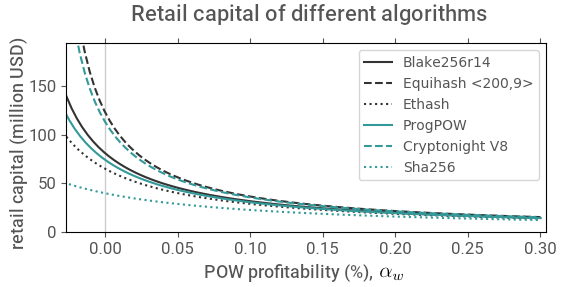
\includegraphics[width=0.80\textwidth]{algo-pcoa}
\begin{minipage}[t]{0.85\textwidth}
	\caption{The difference in PCA between mining algorithms is more significant at low profitabilities. Those algorithms that maximize $ p_d / \omega_d $ have higher PCA across the range of profitabilities.}
	\end{minipage}
  	\end{center}
\hrule
\end{figure}
%

From a network security standpoint, the low-profitability condition is more relavent, as it represents a ''steady-state'' equilibrium condition that persists in the absense of market fluctuations or advancements in hashing hardware. 

There is a minimum profitability given in the zero-gross limit of equation \ref{enet},
%
\begin{equation}
\alpha_{w, min} = - \frac{ 0.024 c }{ \eta \rho }
\end{equation}
%
which is a lower asymptotic value for retail capital.

At the time of writing, Decred mining profitability is less than zero ($ \alpha_w = \num{-2.7e-4} $), resulting in a PCA higher than the ''steady-state'' condition. This is the ideal state for a blockchain. It indicates a good short-term outlook among miners, as the only way to recoup electricity expenditures is if the exchange rate goes up. 

Maximizing the device factor, $ p_d / \omega_d = \eta \rho $, can raise the PCA, as well as the minimum profitability. Further investigation may seek algorithms or alternative consensus mechanisms which can use more hardware but less power.

\subsection{What is the best split of the block reward?}

Transient behavior associated with an abrupt change to a blockchain parameter would be difficult to predict. Long-term behavior in a stable market is easier. If we stick to the assumptions layed out so far about mining profitability and stake returns, then ''steady-state'' conditions can be predicted. 

The stake split, $ s_s $, of $ R_{tot} $ imposes conditions on the treasury split, $ s_t $, and the miner split, $ s_w, $ by the relation $ s_t + s_s + s_w = 1 $. The treasury split is left at 0.1 here. 
%
\begin{figure}[b!]
\vspace{5pt}
\hrule
\vspace{10pt}
	\begin{center}
	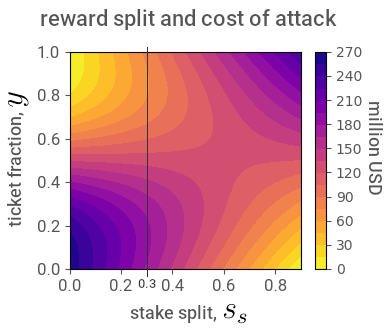
\includegraphics[width=0.60\textwidth]{stakesplit}
\begin{minipage}[t]{0.85\textwidth}
	\caption{The PCA varies with stake split (fraction of block reward given to ticket holders) and stake ownership (portion of ticket pool under attacker control).}
	\end{minipage}
  	\end{center}
\vspace{-15pt}
\end{figure}
%
It is tempting to vary $ s_s $, and consequently $ s_w $, and minimize $ A(y) $ on $ [ 0, 1 ] $ at every point along the way. That approach ignores nuanced economics that would occur if the attacker attempted to purchase a large portion of the ticket pool. How this would affect the stake difficulty can be predicted, but such an action would also presumably spike the exchange rate as the attacker purchased Decred from exchanges to spend on tickets, which is harder to predict. In short, there is more confdence in low-$ y $ predictions than in predictions of the high-$ y $ region. Low-$ y $ conditions also require less time investment from an attacker, as acquiring a significant portion of the stake pool would require a lengthy ticket-buying campaign. 

Figure 5 shows the variation of attack cost with $ y $ and $ s_s $, in the zero-rentability case. The current network configuration of $ s_s = 0.3 $ is a good balance between high entry point at low-$y$, and gradual dropoff at $y > 0.5$. 




% \bibliography{attack}{}
% \bibliographystyle{unsrt}


\begin{appendices}
\section{Network hashrate and POW profitability}



Miner net daily earnings can be written as 
%
\begin{equation}
\label{enet}
E_{net} = \alpha_w p_d = \underbracket{ E_g }_{\text{gross profit}} -  \underbracket{ \frac{ 24 \omega_d c }{ 1000 } }_{ \text{ power costs } } 
\end{equation}
%
which defines a profitability, $ \alpha_w $. The profitability can be thought of as the fraction of device cost retrieved in a day of mining. Profitability self-regulates in that if profitability gets too high, entrepeneurial miners will buy more hashpower and profitability will drop. If profitability drops below zero, it becomes cheaper to buy DCR outright, so miners will turn off their equipment and it will tend back towards zero. 


\begin{figure}[t!]
	\centering
	\vspace{-5pt}
	\hrule
	\vspace{5pt}
	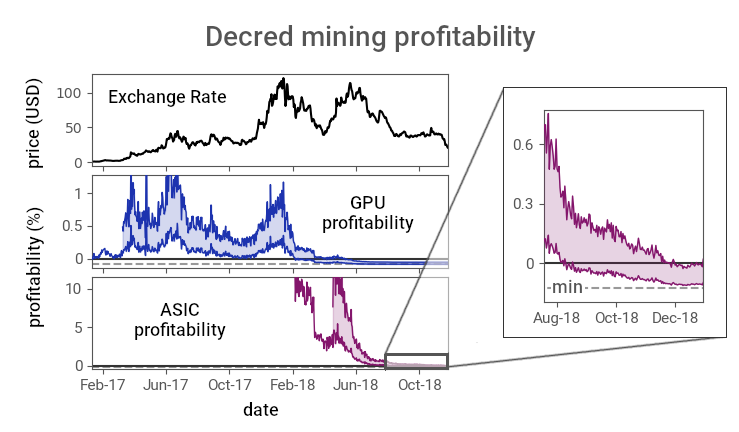
\includegraphics[scale=1.60]{profitability}
	\caption{Mining profitability shows immediate response to price spikes, followed by decay towards zero when the price is stable. \label{profitabilityfig}}
	\vspace{5pt}
\end{figure}

The fiat value of block rewards payed out to miners in a given day can be written in terms of total POW portion of the block reward, $ \beta $ and the fiat exchange rate.
%
\begin{equation}
Q = \beta X
\end{equation}
%

Using the model device statistics, the total number of devices on the network, $ N_d $, can be expressed in two different ways. 
%
\begin{equation}
N_d = \frac{ Q }{ E_{g} } = \frac{ H_{ net } }{ h_d }
\end{equation}
%

Combining this relation with equation \ref{enet}, and substituting alternative device parameters $ \rho $ and $ \eta $, yields an expression for network hashrate. 
%
\begin{equation}
H_{net} = \frac{ \beta X }{ \alpha_w \rho + 0.024 c / \eta  }
\end{equation}
%

\begin{table}[h!]
\footnotesize
\renewcommand{\arraystretch}{1.25}% Spread rows out...
	\vspace{5pt}
	\hrule
	\vspace{6pt}
\begin{tabular}{l|c|c|c|c|}
\cline{2-5}
                                           & \multicolumn{2}{c|}{GPU}                      & \multicolumn{2}{c|}{ASIC}                      \\ \cline{2-5} 
                                           & low                   & high                  & low                   & high                   \\ \hline
\multicolumn{1}{|r|}{$ \eta $ (hashrate		/watt)} & $ 4.1 \times 10^{6} $ & $ 1.8\times 10^{7} $  & $ 3.9\times 10^{8} $  & $ 2.3\times 10^{9} $   \\ \hline
\multicolumn{1}{|r|}{$ \rho $ (\$/hashrate)}   & $ 3.5\times 10^{-7} $ & $ 1.3\times 10^{-7} $ & $ 2.5\times 10^{-9} $ & $ 8.1\times 10^{-10} $ \\ \hline
\end{tabular}
	\caption{Power efficiency, $ \eta $, and relative cost, $ \rho $, of the model devices used for the ranges in figure \ref{profitabilityfig}.}
	\vspace{5pt}
	\hrule
	\vspace{6pt}
\end{table}

\begin{table}[h!]
\footnotesize
\renewcommand{\arraystretch}{1.25}% Spread rows out...
  \begin{tabular}{ | c | c | l | c | c | c | }
    \hline
	\textbf{ algorithm } &\textbf{ Example } &  \textbf{ model device } & \textbf{ price } & \textbf{ hashrate } & \textbf{ power } \\ \hline
	$ Blake256 $ & Decred & D9 Miner &  1699 & \num{2.1e12} & 900  \\ \hline
	$ Cryptonight V8 $ & XMR & 1080 Ti &  475 & 950 & 180  \\ \hline
	$ Equihash(200,9) $ & ZEC & Z9 &  475 & 41,000 & 3300  \\ \hline
	$ Ethash $ & ETH & Antminer E3 &  1150 & \num{ 1.9e8 } & 760  \\ \hline
	$ ProgPOW $ & BCI & 1080 Ti & 475 & 2.2e7 & 275  \\ \hline
	$ SHA256 $ & BTC & Antminer S15 & 1475 & \num{ 2.8e13 } & 1596  \\ \hline
\end{tabular}
	\caption{Model devices for mining algortihms used in section 5.2.}
\end{table}

\newpage

\begin{center}
\small
  \begin{tabular}{ | c | c | l | }
    \hline
	\textbf{ symbol } & \textbf{ unit } & \textbf{ description } \\ \hline
	$ A $ & fiat & \makecell[l]{ Cost of attack. Minimum cost to launch a \\successful attack on the Decred  network. } \\ \hline
	$ a $ & hashes/time & \makecell[l]{Rentability. Amount of hashing power available on\\ the rental market} \\ \hline
	$ \alpha_w $ & $ - $ & \makecell[l]{POW profitability. Daily earnings as a fraction of\\ device cost.} \\ \hline
	$ \alpha_s $ & $ - $ & \makecell[l]{Stake return. Annual percentage yield.} \\ \hline
	$ \beta $ & DCR & \makecell[l]{POW payout. Total decred paid to POW miners\\ per day.} \\ \hline
	$ c $ & fiat/energy & Electricity rate. Common units of \$/kWh. \\ \hline
	$ D $ & fiat & Retail equipment cost. \\ \hline
	$ E_g $ & fiat & Model device gross daily earnings, before power costs. \\ \hline
	$ E_{net} $ & fiat & Model device net daily earnings. \\ \hline
	$ \eta $ & hashrate/power & POW power efficiency. $ \eta = h_d/\omega_d $ \\ \hline	
	$ H_a $ & hash/time & Hashpower required to be under attacker control. \\ \hline
	$ H_{net} $ & hash/time & Total network hashpower. \\ \hline
	$ h_d $ & hash/time & Model device hashrate. \\ \hline
	$ N $ & $ - $ & POS validators per block. \\ \hline
	$ P $ & fiat & Power costs of attack. \\ \hline
	$ p $ & $ - $ & \makecell[l]{Participation level. Fraction of tickets which\\ belong to an online stakeholder.} \\ \hline
	$ p_d $ & fiat & Model device price. \\ \hline
	$ p_t $ & fiat & Ticket price. \\ \hline
	$ \rho $ & fiat/hashrate & Relative device cost. $\rho = p_d / h_d$ \\ \hline
	$ Q $ & fiat & Total POW payout per day, in fiat. \\ \hline
	$ R $ & fiat & Rental costs of attack. \\ \hline
	$ R_{pow} $ & DCR & POW block reward. \\ \hline
	$ R_{tot} $ & DCR & Total block reward. \\ \hline
	$ r_e $ & fiat/hash & Rental rate. \\ \hline
	$ S $ & fiat & Stake term. Total cost of attack spent on tickets. \\ \hline
	$ s_s $ & $ - $ & \makecell[l]{POS rewaard share Fraction of $R_{tot}$. given as a \\stake reward. }\\ \hline
	$ s_w $ & $ - $ & \makecell[l]{ POW reward share. Fraction of $R_{tot} $ given as a \\POW reward. }\\ \hline
	$ \sigma $ & $ - $ & \makecell[l]{ Hashportion. The minimum attacker hashpower, as a \\fraction of total network hashpower.} \\ \hline
  \end{tabular}
\end{center}	

\begin{center}
\small
  \begin{tabular}{ | c | c | l | }
    \hline
	\textbf{ symbol } & \textbf{ unit } & \textbf{ description } \\ \hline
	$ t_a $ & time & Attack duration. Time required to carry out attack. \\ \hline
	$ t_b $ & time & Block time. The network block time target. \\ \hline
	$ W $ & fiat & Work term. Total equipment-related costs of attack. \\ \hline
	$ \omega_d $ & energy/time & Model device power draw. \\ \hline
	$ X $ & fiat/DCR & Exchange rate. \\ \hline
	$ x $ & $ - $ & Hashrate multiplier. \\ \hline
	$ y $ & $ - $ & Attacker controlled fraction of the total stake pool. \\ \hline
	$ Z $ & tickets & Ticket pool size. A network parameter. \\ \hline
  \end{tabular}
\end{center}




\end{appendices}
\end{document}